\subsection{Algorithm}

As both the \gls{hotp} and the \gls{totp} are based on the \gls{hmac} algorithm by building the \gls{otp} over the \gls{hmac} function of the secret key and the counter with a truncation, the underlying \gls{hmac} algorithm needs to be evaluated.\\
The important part here is the chosen cryptographic hash algorithm. Mostly \gls{sha}-1 is used, since it's the default of the RFC. Given that both \gls{sha}-1 and MD5 are considered insecure one has to ask if they are still considered secure in the \gls{otp} context.\\
Because the collision resistance of the chosen cryptographic hash algorithm is not important for the security of the \gls{otp} generation those algorithms do not expose a threat.\\
The \gls{bsi} lists these algorithms as secure for HMAC\footcite{verfahren2019empfehlungen}

Citations: \footcite{10.1007/978-3-319-63688-7_19}

It is more important that the algorithm is implemented correctly, in the past e.g. Google did not issue \gls{otp} values with a leading zero. Besides that, the minimum length of the \gls{otp} values are six digits, meanwhile the RFC supports up to 10.\\
For example Steam, decided to use a different alphabet and character length.

A theoretical vulnerability is to use the time sync offset feature because it enables an attacker to use a token that's much longer valid than it should be. (\textcolor{red}{as discussed in section xx - time sync/drift})

\subsection{Transportation}

Given that the generation of the \gls{otp} is considered secure the more important region to analyze is the transportation of these \gls{otp}. In this section the transportation mediums SMS, E-Mail and App are considered.

\subsubsection{SMS}

The biggest advantage of SMS as a transportation medium is every mobile, ranging from an old Nokia to a new iPhone XS, is capable of receiving SMS. All major mobile phone operation systems come with a SMS application pre-installed, so no external apps are required.\\
SMS are around \textcolor{red}{1999} and highly accepted and easy to use.

While there are some key advantages with SMS transportation it also comes with a lot of downsides. Besides the cost aspect of SMS traffic, both for the sender and potentially for the receiver due to roaming fees, too, the current state of SMS traffic is considered insecure.\\
The SMS traffic relies on the \gls{ss7} network which was developed in the 1970s. It has multiple security flaws that allows an attacker to eavesdrop or modify the in- and out-coming traffic.\footcite{WELCH201717,7997246,puzankov2017stealthy}

In contrast to the web and email the user is not very aware of phishing attacks in the SMS context. Studies however show that a new technique called forward phishing is already in use. In this scenario the attacker sends the victim a (spoofed) SMS from the fakes service provider to reply with the \gls{otp} code for security measures.\footcite{JAKOBSSON20186,SIADATI201714}

Another negative aspect of SMS transportation is the routing. Many companies rely on third-party providers in order to send the SMS to the user. Often these providers like \textcolor{red}{name some} are using countries where SMS are very cheap, but on the other hand the \gls{ss7} security measures like SMS home routing and not enforced. This results in a higher security risk of the SMS being compromised while reaching the user. Also, the third party providers are given access to the \gls{otp} which enables the risk of a malicious insider because the security measures might be weaker than the original company.

Especially for Android there exists multiple SMS trojans which are capable of intercepting the SMS, too.

Given all these facts SMS transportation should be avoided at all costs\footcite{JAKOBSSON20186}, since there are multiple flaws in the \gls{ss7} network itself and the process how the SMS reaches the user. It's also not resistant against phishing or mobile phone trojans.


\begin{figure}[hbt]
	\centering
	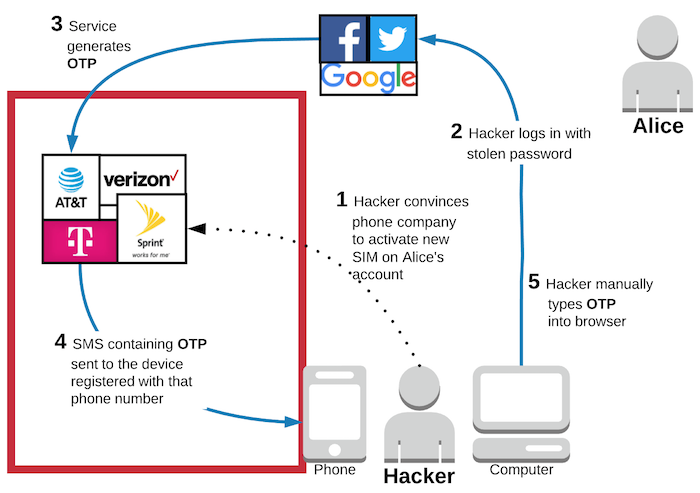
\includegraphics[width=0.8\textwidth]{pics/04---social-engineering-3.png}
	\caption{}
\end{figure}

\begin{figure}[hbt]
	\centering
	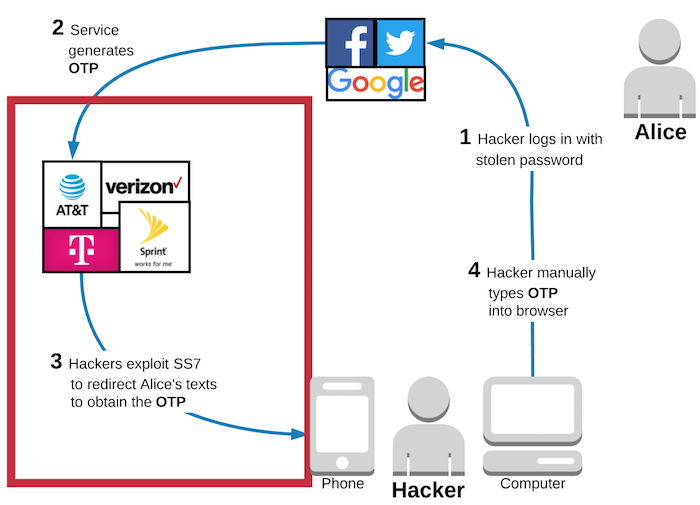
\includegraphics[width=0.8\textwidth]{pics/05---SS7-2.png}
	\caption{}
\end{figure}
% TODO BILDER für Phishing und Interception und Malware}

\subsubsection{cons}

\begin{enumerate}
	\item Delivery time
	\item SIM Swapping, cloning, hijacking, ...
\end{enumerate}

\subsubsection{App}

\subsubsection{pros}

\begin{enumerate}
	\item Works offline
	\item cheaper
\end{enumerate}

\subsubsection{cons}

\begin{enumerate}
	\item Secret can be phished while setup (either on phone or computer)
	\item Trusted apps? OSS? \footcite{eset-bypass2fa}
	\item Vulnerabilities --> e.g. Authy\footcite{sakurity-authy}
\end{enumerate}

\subsubsection{E-Mail}

\subsubsection{pros}

\subsubsection{cons}
